

\chapter{Evaluation}
\label{chapter-evaluation}
Das folgende Kapitel stellt die Evaluation, des im Rahmen dieser Arbeit
realisierten Systems vor. Zunächst werden die Ziele der Evaluation und das
Vorgehen erläutert. Hierbei werden die Versuchsgruppen, welche sich aus der
\nameref{section:benutzer} ergeben, näher betrachtet. Abschließend werden die
Ergebnisse umfassend präsentiert, zusammengefasst und entsprechend diskutiert.

\section{Ziele}
Im Rahmen der Forschungsfrage F3 soll herausgearbeitet werden, inwiefern die
Gebrauchs-tauglichkeit und Nützlichkeit durch das entwickelte Reservierungssystem
gewährleistet werden kann. Die Evaluation wird zusätzlich zur Bewertung
hinsichtlich der Funktion, Gestaltung und Nachvollziebarkeit genutzt, um
Forschungsfrage F2 zu beantworten.


\section{Vorgehen und Methodik}
\todo[inline]{Formative vs. Summative Evaluations https://www.nngroup.com/articles/formative-vs-summative-evaluations/}
Da es sich um ein universitätsinternes Tool handelt, wurde sich zur Evaluation,
im Rahmen einer Laborstudie (N=6) mit Mitarbeitenden des \ac{imis} und
Studierenden im Bereich der Medieninformatik zusammengesetzt. Zu Beginn der
Studienplanung wurden Evaluationsaufgaben definiert, welche die Versuchspersonen
Schritt für Schritt durchführen sollten (\ref{appendix:Evaluation}). Dabei
sollten die Teilnehmenden die Think-Aloud-Methode anwenden. Hierbei werden
Versuchspersonen gebeten, ihre Gedanken während der Nutzung zu verbalisieren
\cite{nielsen_usability_1994}. Als Vorteil gegenüber anderen Methoden werden
Probleme somit nicht nur erfasst, sondern auch begründet\cite{nielsen_think}.

Um die Gebrauchstauglichkeit und Nützlichkeit der Web-App abschließend
feststellen zu können, wurde ein Online-Fragebogen entworfen \todo{Anhang:
  Umfrage}. Zu Beginn des Fragebogens wurden die demografischen Daten der
Teilnehmenden erfasst. Diese dienen der besseren Klassifizierung der Daten.
Daraufhin wurde die Technikaffinität mithilfe der \ac{ati}-Skala erfragt. Im
dritten Abschnitt wurden Fragen zu den Funktionen der Anwendung gestellt.
Hierbei sollte die wahrgenommene Nützlichkeit der Funktionen angegeben und
gewünschte Funktionen genannt werden. Dies dient unter anderem dem Ausblick und
Abwägen der zukünfitgen Weiterentwicklung des Systems. Des Weiteren wurde in
diesem Teil auf die Verwendung verschiedener Begrifflichkeiten innerhalb der
Anwendung eingegangen, da diese in der Zwischenevaluation des
\nameref{chapter-design}s vermehrt zu Unverständlichkeiten geführt haben.
Zusätzlich wurde mithilfe des \ac{ueq} die Gebrauchstauglichkeit getestet
\cite{burghardt_mensch_2018}. Abschließend wurden Proband:innen nach einer
Gesamtbewertung des Systems befragt und ob sie sich die regelmäßige Nutzung
vorstellen könnten.



\section{ATI und UEQ Ergebnisse}
Da sich die Anwendung lediglich im Bereich der Verwaltung unterscheidet, werden im
Folgenden die Technikaffinität und die bewertete Usability der Anwendung beider
Versuchsgruppen dargestellt.

Zur Vollständigkeit sollte die Gebrauchstauglichkeit der Anwendung mithilfe des \ac{ueq} betrachtet
werden. Dieser teilt die Usability des Systems in seine pragmatische und hedonische Qualität auf.
Hierbei beschreibt die pragmatische Qualität die wahrgenommene Fähigkeit eines Systems, Nutzende in
ihrer Aufgabenerledigung effektiv und effizient zu unterstützten \cite{hassenzahl_thing_2004}. Die
hedonische Qualität bezieht sich hingegen auf die emotionalen und ästhetischen Bestandteile eines
Systems. So wird beispielsweise die Erfüllung menschlicher Bedürfnisse nach Neugier und sozialem
Vergleich erfasst \cite{hassenzahl_thing_2004}.

Werte zwischen -0.8 und 0.8 stehen für eine neutrale Bewertung der entsprechenden Skala. Somit
stehen Werte größer als 0.8 für eine positive Bewertung und Werte kleiner als -0.8 für eine negative
Bewertung. Der Bereich der Skalen liegt zwischen -3 (sehr schlecht) und +3 (sehr gut). Für die
Interpretation der Ergebnisse sollte beachtet werden, dass kein Vergleichsystem vorliegt. Die
Aussagekraft der ausgewerteten Ergebnisse ist somit zu hinterfragen.

\begin{table}[h]
  \centering
  \caption{Werte der kurzen \ac{ueq}-Skala}
  \begin{tabular}{lc}
    \arrayrulecolor{maincolor}\hline
    Pragmatische Qualität & 1.75 \\
    Hedonsiche Qualität   & 0.75 \\
    Gesamt                & 1.25 \\
    \arrayrulecolor{maincolor}\hline
  \end{tabular}
  \label{table:ueq}
\end{table}

\todo{muss Abb. 7.1 ? Wenn muss das noch hübsch :D}
\begin{figure}[h]
  \centering
  \caption{EQ}
  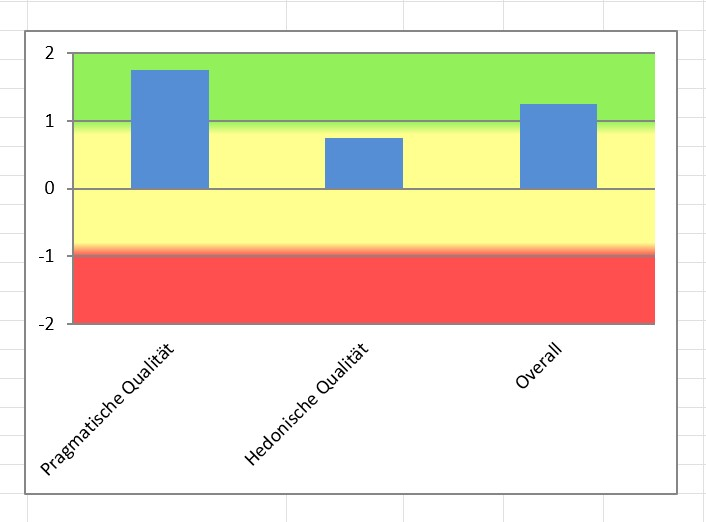
\includegraphics[scale=0.7]{Bilder/Screenshot 2022-10-26 165800.jpg}
  \caption[UEQ]{Verzeichn}
  \label{fig:ueq}
\end{figure}

Des Weiteren wurde mithilfe des \ac{ati} das technische Interesse und
Verständnis der Teilnehmenden festgestellt (\ref{table:ati})
\cite{attig_assessing_2017}. In beiden Gruppen konnten wie zu Beginn in der
\refname{section:benutzer} lediglich geringe Unterschiede innerhalb der
soziodemografischen Daten festgestellt werden.

Insgesamt konnte für beide Gruppen eine Einschätzung der Technikaffinität anhand
der \ac{ati}-Skala ermittelt werden (Verleihende: M=5.XX, SD=0.XX, N=3;
Ausleihende: M=5.XX, SD=0.XX, N=X) (\ref{table:ati}). Durch die Hinzunahme
zweier Vergleichsstichproben aus \citeA{franke_personal_2019} (M=4.14, N=300 und
M=4.23, N=65), lässt sich schlussfolgern, dass die Nutzendengruppen eine
vergleichsweise hohe Technikaffinität aufweisen.


\begin{table}[h]
  \centering
  \caption{Werte der \ac{ati}-Skala}
  \begin{tabular}{lccc}
    \arrayrulecolor{maincolor}\hline
    \sffamily\color{maincolor}Benutzergruppe            &
    \sffamily\color{maincolor}Mittelwert $(M)$          &
    \sffamily\color{maincolor}Standardabweichung $(SD)$ &
    \sffamily\color{maincolor}Teilnehmende $(N)$                        \\
    \arrayrulecolor{maincolor}\hline
    Verleihende                                         & 5.X & 0.X & 3 \\
    Ausleihende                                         & 5.X & 0.X & 8 \\
    \arrayrulecolor{maincolor}\hline
  \end{tabular}
  \label{table:atipartzwei}
\end{table}


\section{Verleihende}
Der kommende Abschnitt umfasst aus Sicht der Verleihenden lediglich die Evaluationsergebnisse der
Aufgaben in Bezug auf den Verwaltungsteil des realisierten Systems.
\ref{table:vzwei} zeigt die Rollen der Versuchspersonen. Die IDs der Versuchspersonen werden als
Verweise in dem folgenden Abschnitt verwendet.

\begin{table}[h]
  \centering
  \caption{Teilnehmende der Interviews, Verleihende}
  \begin{tabular}{lll}
    \arrayrulecolor{maincolor}\hline
    \sffamily\color{maincolor}ID &
    \sffamily\color{maincolor}Zuständigkeitsbereich \\
    \arrayrulecolor{maincolor}\hline
    E-V1                         & Multimedialabor  \\
    E-V2                         & VR-Labor         \\
    E-V3                         & ??               \\
    \arrayrulecolor{maincolor}\hline
  \end{tabular}
  \label{table:vzwei}
\end{table}

Für Verleihende ist es von hoher Bedeutung überprüfen zu können, ob die richtige
Person das entsprechende Asset abholt. Dies wurde nach dem Klicken auf das
Listenelement erwartet (E-V1). Des Weiteren bedarf die Bestätigung, dass ein
Asset \textit{abgeholt} oder \textit{zurückgegeben} wurde, bei mehreren
Elementen in der Listenansicht, viele Aktionen. Folglich wurde eine
Bearbeitungsansicht beim Klicken des Listenelements erwartet oder vorgeschlagen
(E-V1-2).

\begin{longtable}{p{0.85\textwidth}} \arrayrulecolor{maincolor}\hline
  \enquote{\textit{\enquote{Abgeholt}, dass muss man bestätigen können. Wenn ich
  da ausversehen raufklicke [\dots] wichtig ist eine undo-Oberfläche [\dots]
  keine Ahnung wie ich das jetzt zurückhole [\dots]}} \\
  \arrayrulecolor{maincolor}\hline
\end{longtable}

\section{Ausleihende}

Der kommende Abschnitt umfasst die Evaluationsergebnisse der Aufgaben, unter der
Anwendung der Think-Aloud-Methode, aufseiten der Ausleihenden. \ref{table:azwei}
zeigt die Rolle und das Alter der Versuchspersonen. Die IDs der Versuchspersonen
werden als Verweise in dem folgenden Abschnitt verwendet.

\begin{table}[h]
  \centering
  \caption{Teilnehmende der Evaluation, Ausleihende}
  \begin{tabular}{lll}
    \arrayrulecolor{maincolor}\hline
    \sffamily\color{maincolor}ID & \sffamily\color{maincolor}Alter &
    \sffamily\color{maincolor}Rolle                                  \\
    \arrayrulecolor{maincolor}\hline
    E-A1                         & 19 - 25 J.                      &
    Masterstudent:in, Hilfswissenschaftlerin:in                      \\
    E-A2                         & 19 - 25 J.                      &
    Bachelorstudent:in                                               \\
    E-A3                         & 19 - 25 J.                      &
    Bachelorstudent:in, Hilfswissenschaftler:in                      \\
    E-A4                         & 19 - 25 J.                      &
    Bachelorstudent:in, Hilfswissenschaftler:in                      \\
    E-A5                         & 19 - 25 J.                      &
    Masterstudent:in                                                 \\
    \arrayrulecolor{maincolor}\hline
  \end{tabular}
  \label{table:azwei}
\end{table}

Auf dem Einloggbildschirm wurde der Name der Anwendung erwartet, da die
Zuordnung des Tools sonst schwerfallen könnte. Außerdem war die Wortwahl und der
Platz zum \textit{Mit IDM Accout einloggen}-Button problematisch, da die
Eingabefelder und der Button als zwei unterscheidliche Einlogg-Wege verstanden
wurden und nicht als Bestätigungs-Button für das Formular (E-V1, E-A4).

Das Dashboard wurde von den Nutzenden stets als übersichtlich und hilfreich
betitelt, wobei die Namensgebung \textit{Dashboard} als einziges englisches
Wort negativ aufgefallen ist (E-V1). In der Beschreibung der Tabs würde ein
\textit{deine} förderlich sein, um zu verdeutlichen, dass es sich um die eigens
getätigten Reservierungen handelt und nicht um alle Reservierungen (E-A1). Da
das Dashboard bei keinen Reservierungen viel freien Platz lässt, wäre eine
direkte Übersicht über Kategorien denkbar sinnvoll (E-A3).

Die Kategorien wurden von allen Nutzenden als einfach und wichtig bezeichent.
Positiv wurde angemerkt, dass diese ein schnelles Durchsuchen ermöglichen, um zu
erfahren, was für Materialien ausgeliehen werden können (E-A3). Ohne Kategorien
sei die Anwendung nur halb so übersichtlich (V-E4).

\begin{longtable}{p{0.85\textwidth}} \arrayrulecolor{maincolor}\hline
  \enquote{\textit{[\dots], die Kategorien das hätte ich mir nur ein bisschen
      übersichtlicher gewünscht, [\dots] und vielleicht auf dem Dashboard schon eine
  Art Übersicht.}} \\
  \arrayrulecolor{maincolor}\hline
\end{longtable}

Eine weitere Beobachtung, in Hinsicht auf die Kategorien, betrifft das
aufgeklappen der Unterkateogien. Nachdem diese geöffent wurden müssen Nutzende
zunächt auf \textit{zurück}-klicken, um Oberkategorien erneut einsehen zu können
(V-E3).

Allen Versuchspersonen ist das Suchen über die Sucheleiste sowie die
Navigationsleiste leicht gefallen. Ansprechpartner:innen und der Abholort eines
Assets wurden auf den ersten Blick entdeckt. Wobei eine Raumnummer bei dem
Abholort als fehlend deklariert wurde.

\begin{longtable}{p{0.85\textwidth}} \arrayrulecolor{maincolor}\hline
  \enquote{\textit{[\dots], wenn hier die Kontaktdaten zu den Verantwortlichen
      sind [\dots], dass man draufklicken könnte und direkt kontaktieren könnte
  über die App [\dots]}} \\
  \arrayrulecolor{maincolor}\hline
\end{longtable}

Suche über die Navigationsleiste wurde als modern und ansprechend befunden. Die
Suche im Burgermenü wurde nicht von allen Nutzenden als eindeutig und hilfreich
betitelt (E-??). Das Suchen über einen bestimmten Zeitraum erschien sehr praktisch
(E-A5). Ergänzend könnte in der Navigationsleiste ein Filtericon eingebaut
werden, welches ebenfalls das Suchen über einen Zeitraum beinhaltet (E-A5).

Der Reservierungsprozess wurde durch die Kalenderkomponente zu Teilen erschwert. Als irritierend
galt die fehlende Hervorhebung des aktuellen Tages (E-A1,2). Nicht auswählbare Tage werden bisher
lediglich ausgegraut, was die Unterscheidung zwischen generell nicht auswählbaren Tagen (Wochenende)
und bereits reservierten Zeiträumen unübersichlich wirken lässt. Die Kalender und Uhrzeitenansicht
wurde bis dato auf Englisch angezeigt, wobei Versuchspersonen anmerkten, dass diese auf Deutsch für
die Einheitlichkeit sinnvoller wären (E-A1). Sobald der Zeitraum ausgewählt wurde, erhielten
Nutzende eine Reservierungsübersicht und eine Zusammenfassung. Die Bestätigung von zwei
Reservierungsübersichten war für die Versuchsperson unklar. Bereits bei der ersten Übersicht
interpretierten Nutzenden die Reservierung als abgeschlossen, einige kehrten zum Dashboard zurück,
wo die Reservierung jedoch nicht angezeigt wurde. Dieses Missverständnis wurde unter anderem auf die
Betitelung des Butten \textit{weiter} zurückgeführt. Um den Reservierungsprozess sichtbarer zu
gestalten, wurde Vorschlag eine Fortschrittsanzeige einzublenden (E-A3). Ein weiterer Punkt,
weswegen das Abschließen der Reservierung als (nicht)entgültig interpretiert werden kann, ist das
Fehlen eines \textit{Zurück zum Dashboard}-Button auf der Reservierungszusammenfassung (E-A1,3). Des
Weiteren hat die Animation der Kalenderkomponente beim Schließen dieser als Bestätigung
interpritiert (E-V1, A3).

Um erneut Informationen zum reservierten Material einsehen zu können, erschien es
als umständlich, dass Nutzende erneut nach dem Material suchen müssen. Alle
Versuchspersonen haben intuitiv auf das im Dashboard angezeigte Listenelement
geklickt und eine Verlinkung erwartet (E-V1 bis E-V5, E-A1-2). Eine
Versuchsperson hat zunächst auf das Listenelement geklickt, in der Erwatung,
dass sich eine Seite zum Bearbeiten des Materials öffnet (E-A4). Beim Bearbeiten
des Zeitraums stellte sich das Kalender-Popup, auf der mobile Version, als
unhandlich heraus, da sich automatisch die Tastatur öffnet und die Komponente
sich beim Danebentippen direkt wieder schloss. Außerdem fehlte eine Bestätigung
der Änderung oder ein \textit{Änderungen speichern}-Button (E-A1 bis 5, E-V1-2).
Ebenfalls wurde von allen Versuchspersonen die im Kalender ausgewählten Tage per
Ziehen versucht zuverändert.

Das Löschen einer Reservierung hat bei allen Versuchspersonen gut funktoniert
und wurde als intuitiv bezeichnet. Zwei Personen wiesen darauf hin, dass vor dem
Löschen eine Warnung sinnvoll ist, falls Nutzende ausversehen auf Löschen
klicken (V-E1. E-A1).

Die Assetstatus \textit{Fest verbaut} und \textit{Am Standort nutzbar} führten
bei den Versuchspersonen zu Irritation. Versuchspersonen fehlte zu der Betitelung
eine Erkläurng.\todo{Wording oder legende.}

\begin{longtable}{p{0.85\textwidth}} \arrayrulecolor{maincolor}\hline
  \enquote{\textit{Was bedeutet das für die Reservierung?}} \\
  \enquote{\textit{[\dots] das heißt von \enquote{fest verbaut} frage ich mich,
      ob ich das jetzt trotzdem ausleihen kann oder ob \enquote{fest verbaut} heißt,
  dass ich dass nur vor Ort nutzen kann[\dots]}}            \\
  \enquote{\textit{[\dots] das (der Assetstatus) könnnte vielleicht ein bisschen
  salienter sein.}}                                         \\
  \arrayrulecolor{maincolor}\hline
\end{longtable}

Generell wurde die Oberfläche als übersichtlich und \textit{clean} beschrieben
(E-A1 bis E-A4). Der Wunsch, die Anwendung im Universitätsalltag für Projekte
nutzen zu können, wurde entsprechend geäußert (E-A1,3,4).

\begin{longtable}{p{0.85\textwidth}} \arrayrulecolor{maincolor}\hline
  \enquote{\textit{Ja, wäre cool, wenn wir das am IMIS wirklich nutzen
  könnten}}                                                      \\
  \enquote{\textit{[\dots] es ist insgesamt sehr übersichtlich und ich würde
  sagen, dass ich mich auf jeden Fall gut zurechtfinde [\dots]}} \\
  \enquote{\textit{Allgemein die Idee, dass es wie ein Online-Shop ist [...] ,
      weil viele Leute einfach alles neu kaufen, statt es auszuleihen und wenn du
      denen einen Online-Shop an die Hand gibts, können die einfach [\dots] danach
  suchen.}}                                                      \\
  \arrayrulecolor{maincolor}\hline
\end{longtable}


\begin{itemize}
  \item Anhang
  \item Keine Funktion als unötig geschrieben
  \item Suche und auch das Reservieren = Zentrall
  \item Im Verhältnis die Kachelübersicht nicht so zentrale
  \item deckungsgleich mit Think aloud aussagen
\end{itemize}


\section{Diskussion}